\documentclass[11pt]{article}

% ---------------------------------------------------------------
% polilabs --- An Architecture Walkthrough
% Companion file: polilabs-graph.html (interactive Figure 2)
% Build:  tectonic polilabs-architecture.tex
%    or:  pdflatex (x3)
% ---------------------------------------------------------------

\usepackage[T1]{fontenc}
\usepackage[utf8]{inputenc}
\usepackage{charter}
\usepackage[scaled=0.92]{helvet}
\usepackage[scaled=0.85]{beramono}
\usepackage[margin=1in]{geometry}
\usepackage{xcolor}

% ---- palette (matches polilabs-graph.html) -------------------
\definecolor{cJur}{HTML}{475569}
\definecolor{cBill}{HTML}{1E40AF}
\definecolor{cVer}{HTML}{3B82F6}
\definecolor{cSec}{HTML}{0D9488}
\definecolor{cTerm}{HTML}{16A34A}
\definecolor{cStat}{HTML}{D97706}
\definecolor{cAmend}{HTML}{DC2626}
\definecolor{cSpon}{HTML}{7C3AED}
\definecolor{ink}{HTML}{1C1B19}
\definecolor{ink2}{HTML}{55514A}
\definecolor{rule}{HTML}{D8D4CA}
\definecolor{panel}{HTML}{F4F2EC}

\usepackage{booktabs}
\usepackage{enumitem}
\usepackage{tikz}
\usetikzlibrary{arrows.meta,positioning,fit,backgrounds,calc}
\usepackage{microtype}
\usepackage[colorlinks=true,linkcolor=cBill,urlcolor=cBill,citecolor=cBill]{hyperref}

\setlength{\parskip}{0.55em}
\setlength{\parindent}{0pt}
\sloppy

% ---- helpers -------------------------------------------------
\newcommand{\code}[1]{{\ttfamily\small #1}}
\newcommand{\nodet}[2]{{\color{#1}\sffamily\bfseries #2}}
\newcommand{\sectionrule}{\vspace{-0.6em}{\color{rule}\hrule height 1pt}\vspace{0.4em}}

\title{\vspace{-1.2cm}\textbf{\textsf{polilabs}}\\[0.2cm]
  {\Large An Architecture Walkthrough}\\[0.15cm]
  {\normalsize\color{ink2}The corpus, the knowledge graph, the agent tools ---
   and who it is for}}
\author{\textsf{\small Internal engineering documentation}}
\date{\textsf{\small \today\quad$\cdot$\quad companion file: \code{polilabs-graph.html}}}

\begin{document}
\maketitle
\thispagestyle{empty}

\begin{center}
\begin{minipage}{0.9\textwidth}
\small\color{ink2}
\textbf{How to read this.} Sections~1--5 explain the machine: what is in the
corpus, how a pile of bills becomes a queryable graph, and how an AI agent
asks it questions. Section~6 steps back to the human side --- who actually
uses legislative research and how. Section~7 is an honest status report.
The companion file \code{polilabs-graph.html} is the live, clickable version
of Figure~\ref{fig:graph}; open it side by side.
\end{minipage}
\end{center}

\vspace{0.3cm}
\sectionrule

\tableofcontents
\vspace{0.4cm}
\sectionrule

% =================================================================
\section{What polilabs is}

polilabs is an \textbf{agent-native, queryable knowledge graph of US federal
legislation}. The version~1 corpus is \textbf{191 AI-governance bills} from the
118th and 119th Congresses (2023--2026).

The single most important framing point is this: \emph{the product is not the
data}. Anyone can download bill text from Congress.gov. The product is the
\textbf{interface} --- a set of precise, machine-friendly query primitives that
let an AI agent investigate the corpus without making things up. polilabs is the
backend; the agent doing the research is \emph{yours} (Claude, a Cursor
session, a custom app), not polilabs' own.

\subsection{The problem it exists to solve}

Commercial legal-AI tools hallucinate. Not occasionally --- measurably. A 2024
Stanford study (Magesh et al.) found purpose-built legal AI products produced
hallucinated answers in \textbf{17--34\%} of queries; a companion paper (Dahl et
al., \emph{Large Legal Fictions}) found near-chance accuracy on questions about
whether two legal sources agree.

The polilabs wager is that this happens not because language models are
hopeless, but because the \emph{substrate} they reason over is hostile to
machines. Legislative text is written for trained humans with a keyword-search
box. Hand an agent a search box and ask ``does bill X conflict with bill Y''
and it will confabulate --- because nothing in the substrate lets it
\emph{traverse} from X to Y along a typed, verifiable path.

polilabs rebuilds the substrate. It does three things a raw pile of XML cannot:

\begin{enumerate}[leftmargin=1.4em,itemsep=2pt]
\item \textbf{Reconciliation.} Bill metadata (Congress.gov), full text
  (GovInfo), and references to existing law (US Code) are stitched into one
  graph. Each \code{sources/*} client is deliberately thin --- the value is the
  stitching, not the fetching.
\item \textbf{Agent-native primitives.} A question like ``which bills define
  \emph{foundation model}'' is \emph{one} tool call, not fifty. The tool set is
  designed against documented LLM failure modes (the ``N+1'' search-then-loop
  pattern, context degradation, pagination truncation).
\item \textbf{Anti-hallucination by construction.} Every fact an agent can
  retrieve carries verbatim provenance. Definitions are scoped to the bill that
  defines them --- there is no global ``AI'' node --- so an agent reporting a
  definition physically cannot blend two bills together.
\end{enumerate}

% =================================================================
\section{The corpus}

\subsection{What is in it}

The v1 corpus is a curated, version-controlled set of 191 bills. ``Curated''
matters: this is not every bill that mentions AI, it is the set that survived an
explicit inclusion test (Section~2.3).

\begin{table}[ht]
\centering\small
\begin{tabular}{@{}lr@{\hskip 2.2em}lr@{}}
\toprule
\textbf{Dimension} & \textbf{Count} & \textbf{Dimension} & \textbf{Count}\\
\midrule
Bills (total)            & 191  & House bills (\code{hr})        & 109\\
118th Congress (2023--24)& 100  & Senate bills (\code{s})        & 81\\
119th Congress (2025--26)& 91   & Concurrent resolution         & 1\\
Tier A (AI is headline)  & 184  & Sections (graph nodes)        & 29{,}616\\
Tier B (AI is a part)    & 7    & Defined terms                 & 1{,}241\\
Cosponsor links          & 688  & Amendment operations          & 190\\
\bottomrule
\end{tabular}
\caption{The v1 corpus at a glance. Date span of introduction: 2023-01 to
2026-05.}
\end{table}

\textbf{Subject.} Every bill is AI-governance legislation. The largest policy
areas are \emph{Science, Technology, Communications} (62 bills), \emph{Government
Operations} (31), \emph{Armed Forces and National Security} (22), and
\emph{Commerce} (19) --- AI policy is not one committee's problem, it is spread
across the whole legislative map.

\textbf{Streams.} The corpus is partitioned by \emph{type of legal instrument}.
Only the \code{legislation} stream (bills and resolutions) is in v1 scope.
The \code{regulatory} stream (FTC, NIST, Commerce actions) and the
\code{executive} stream (executive orders) are deliberately out of scope and
kept in separate buckets --- they are \emph{never} silently merged in. This is
itself an anti-hallucination decision: an agent must be able to say ``executive
orders are outside this corpus'' rather than guess.

\textbf{Tiers.} Each bill carries a \emph{centrality tier}. Tier~A means AI is
the headline subject (the title or summary makes AI policy the core purpose).
Tier~B means AI is a substantial part but not the headline --- e.g.\ a defense
authorization bill with an AI title. Tier~C (AI mentioned only in passing)
is defined only to mark the \emph{exclusion} boundary: Tier~C bills never enter
the corpus.

\subsection{Anatomy of a bill on disk}

The corpus is plain files, committed to the repository. Each bill is one
directory under \code{data/corpus/legislation/}, named by its canonical id:

\begin{center}\small
\code{data/corpus/legislation/118-hr-6881/}
\end{center}

\begin{table}[ht]
\centering\small
\begin{tabular}{@{}lp{10.4cm}@{}}
\toprule
\textbf{File} & \textbf{What it holds}\\
\midrule
\code{metadata.json}   & Reconciled bill metadata: title, sponsor, cosponsors,
  introduced date, policy area, every legislative action, the list of available
  text versions, the chosen canonical version, the centrality score and tier.\\
\code{bill.xml}        & The full legislative text, as legislative XML (USLM, or
  the older ``pre-USLM'' dialect). This is the authoritative text.\\
\code{bill.htm}        & The same text as human-readable HTML (a convenience copy).\\
\code{provenance.json} & The audit trail: the exact source URLs (GovInfo XML,
  GovInfo HTML, Congress.gov), the package id of the version used, and the UTC
  fetch timestamp. Every fact in the corpus traces back through this file.\\
\bottomrule
\end{tabular}
\caption{The four-file layout of every bill. 191 directories, identical shape.}
\end{table}

\textbf{The id scheme.} A bill's canonical id is
\code{\{congress\}-\{type\}-\{number\}} --- e.g.\ \code{118-hr-6881},
\code{118-s-4178}. Inside the graph the same bill is addressed as a URN:
\code{bill:us/118/hr/6881}. A section within a bill is
\code{\{bill\}::\{xml\_id\}}, where \code{xml\_id} is the stable identifier the
legislative XML already carries. The API accepts every form and normalizes at
the boundary.

\textbf{Inside \code{bill.xml}.} A bill is a nested tree. The body
(\code{<legis-body>}) contains \code{<section>} elements, each of which contains
\code{<subsection>}, \code{<paragraph>}, \code{<subparagraph>},
\code{<clause>}\ldots\ each level carrying an \code{<enum>} (its label: ``1.'',
``(a)'', ``(1)''), a \code{<header>} (its heading), and \code{<text>} (the
verbatim provision). Cross-references to existing law appear inline as
\code{<external-xref>} elements. This nested-enum tree, with its stable ids, is
exactly what becomes the \nodet{cSec}{Section} nodes of the graph.

\subsection{How bills got in: the ingest pipeline}

The corpus is not hand-picked. It is the output of a four-stage pipeline
(\code{ingest/}), and the pipeline's selectivity is the point.

\begin{enumerate}[leftmargin=1.5em,itemsep=3pt]
\item \textbf{Discover.} Full-text search against the GovInfo \code{BILLS}
  collection over the date range, with a deliberately \emph{wide} term net
  (``artificial intelligence'', ``machine learning'', ``generative AI'',
  ``automated decision systems'', ``facial recognition''\ldots). Cast wide now;
  filter strictly later.
\item \textbf{Score.} Each unique bill is run through a hard \emph{anchor gate}:
  it must contain ``artificial intelligence'', ``machine learning'', or the
  standalone token ``AI'' in a meaningful field. No anchor $\Rightarrow$ out,
  no matter how AI-adjacent it looks. Survivors get a \emph{centrality score}:
  a weighted sum over where the anchor terms appear (a hit in the title counts
  4$\times$ a hit in the summary).
\item \textbf{Reconcile.} For each survivor, rich metadata is pulled from
  Congress.gov --- sponsor, cosponsors, actions, policy area, official summary
  --- and cross-checked against the GovInfo text. ``Cross-check, don't wrap.''
\item \textbf{Promote.} Bills scoring above threshold (or marked include by a
  human reviewer) are materialized into the four-file directory layout, and the
  corpus index is written.
\end{enumerate}

The funnel is real: \textbf{279 candidate bills were discovered; 191 were
promoted.} The other 88 fell below the centrality threshold. The pipeline is
re-runnable and idempotent, so the corpus can be refreshed or expanded without
disturbing what is already in.

% =================================================================
\section{From documents to a graph}

A directory of XML files is authoritative but not queryable. Turning it into
something an agent can traverse is the engineering core of polilabs. It happens
in \emph{two} stores, built side by side from the same source.

\subsection{Two stores, and why}

\begin{table}[ht]
\centering\small
\begin{tabular}{@{}lp{5.1cm}p{5.6cm}@{}}
\toprule
 & \textbf{SQLite} (\code{polilabs.db}) & \textbf{K\`uzu graph} (\code{polilabs.kuzu})\\
\midrule
\textbf{Shape}    & Relational tables + full-text search index & Property graph: typed nodes, typed edges\\
\textbf{Good at}  & ``Find bills mentioning X'' --- fast keyword discovery; bill and section metadata & ``What connects to what'' --- definitions, citations, amendments, cross-bill links\\
\textbf{Holds}    & \code{bills}, \code{sections}, \code{cosponsors}, \code{actions}; two FTS5 search indexes & \code{Bill}, \code{Section}, \code{DefinedTerm}, \code{StatuteSection}, \code{AmendmentOperation}\ldots\\
\bottomrule
\end{tabular}
\caption{The two stores. Both are \emph{embedded} (in-process, no server, like a
file) and both are regenerated destructively from \code{data/corpus/}. They are
not redundant: discovery wants a search index, structural reasoning wants a
graph.}
\end{table}

Both are derived; neither is a source of truth. Delete them and they rebuild
from the corpus in about a minute. Figure~\ref{fig:pipeline} shows the whole
path.

\begin{figure}[ht]
\centering
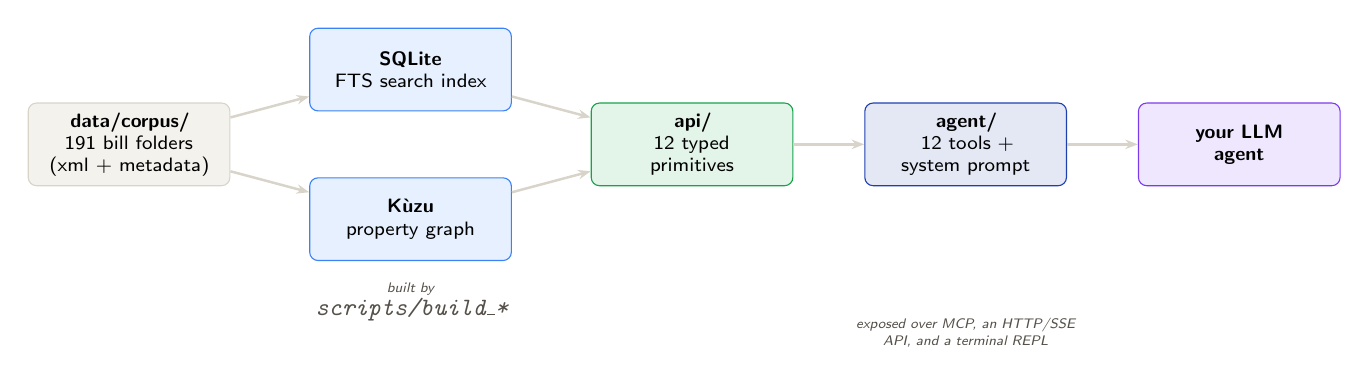
\begin{tikzpicture}[
  font=\sffamily\scriptsize,
  box/.style={draw=rule,fill=panel,rounded corners=3pt,minimum height=1.05cm,
    text width=2.35cm,align=center,inner sep=3pt},
  store/.style={box,fill=cVer!12,draw=cVer},
  arr/.style={-{Stealth[length=1.6mm]},rule,line width=0.9pt},
  node distance=0.7cm]
\node[box] (corpus) {\textbf{data/corpus/}\\191 bill folders\\(xml + metadata)};
\node[store,right=1.0cm of corpus,yshift=0.95cm] (sql) {\textbf{SQLite}\\FTS search index};
\node[store,right=1.0cm of corpus,yshift=-0.95cm] (kuzu) {\textbf{K\`uzu}\\property graph};
\node[box,right=1.0cm of sql,yshift=-0.95cm,fill=cTerm!12,draw=cTerm] (api)
  {\textbf{api/}\\12 typed\\primitives};
\node[box,right=0.9cm of api,fill=cBill!12,draw=cBill] (tools)
  {\textbf{agent/}\\12 tools +\\system prompt};
\node[box,right=0.9cm of tools,fill=cSpon!12,draw=cSpon] (agent)
  {\textbf{your LLM}\\\textbf{agent}};
\draw[arr] (corpus) -- (sql);
\draw[arr] (corpus) -- (kuzu);
\draw[arr] (sql) -- (api);
\draw[arr] (kuzu) -- (api);
\draw[arr] (api) -- (tools);
\draw[arr] (tools) -- (agent);
\node[font=\sffamily\tiny\itshape,below=0.15cm of kuzu,text width=2.5cm,
  align=center,text=ink2] {built by\\\code{scripts/build\_*}};
\node[font=\sffamily\tiny\itshape,below=1.55cm of tools,text width=3.2cm,
  align=center,text=ink2] {exposed over MCP, an HTTP/SSE\\API, and a terminal REPL};
\end{tikzpicture}
\caption{The pipeline. The corpus is the source of truth; everything to its
right is derived and regenerable.}
\label{fig:pipeline}
\end{figure}

\subsection{The node types}

The graph has ten node types that are populated in v1. Think of them in three
groups: the \emph{bibliographic} backbone (the bill as a document), the
\emph{substantive} layer (what the bill says and does), and the
\emph{provenance} spine (who derived what).

\begin{table}[ht]
\centering\small
\begin{tabular}{@{}llp{7.0cm}r@{}}
\toprule
\textbf{Node} & \textbf{Group} & \textbf{What it is} & \textbf{Count}\\
\midrule
\nodet{cJur}{Jurisdiction}    & biblio & The sovereign (here: the United States) & 1\\
\nodet{cBill}{Bill}           & biblio & The bibliographic record of one bill & 191\\
\nodet{cVer}{BillVersion}     & biblio & A dated text snapshot at one procedural stage & 191\\
\nodet{cSec}{Section}         & biblio & A node in the bill's body tree (section\ldots clause) & 29{,}616\\
\nodet{cSpon}{Sponsor}        & biblio & A legislator who (co)sponsors a bill & 411\\
\nodet{cTerm}{DefinedTerm}    & subst. & A term a section formally defines & 1{,}241\\
\nodet{cStat}{StatuteSection} & subst. & A section of existing US Code a bill touches & 172\\
\nodet{cAmend}{AmendmentOperation} & subst. & One reified edit to existing law & 190\\
Extractor                     & prov.  & A parser that derived edges & 4\\
ProvenanceRecord              & prov.  & One record of an extractor run & 4\\
\bottomrule
\end{tabular}
\caption{The populated node types. (Three further types ---
\code{Committee}, \code{Statute}, \code{UnresolvedTermUse} --- are declared in
the schema but not yet populated; see Section~7.)}
\end{table}

\subsection{The edge types --- and how each is derived}

Edges are where the value is. Each is \emph{typed} (it has a name and a fixed
source/target), and each is \emph{derived mechanically} from the source XML ---
no language model invents an edge.

\begin{table}[ht]
\centering\footnotesize
\begin{tabular}{@{}llp{6.9cm}r@{}}
\toprule
\textbf{Edge} & \textbf{From $\rightarrow$ To} & \textbf{How it is derived} & \textbf{Count}\\
\midrule
\code{OF\_JURISDICTION} & Bill $\rightarrow$ Jurisdiction & Every bill, mechanically & 191\\
\code{HAS\_VERSION}     & Bill $\rightarrow$ BillVersion  & From the chosen canonical version & 191\\
\code{HAS\_SECTION}     & BillVersion $\rightarrow$ Section & Each top-level section of the body & 647\\
\code{PARENT\_OF}       & Section $\rightarrow$ Section    & The nesting of the body tree & 28{,}969\\
\code{SPONSORED\_BY}    & Bill $\rightarrow$ Sponsor      & From the bill's sponsor field & 191\\
\code{COSPONSORED\_BY}  & Bill $\rightarrow$ Sponsor      & From the cosponsor list & 688\\
\code{DEFINES}          & Section $\rightarrow$ DefinedTerm & Sections under a ``Definitions'' heading & 1{,}244\\
\code{BY\_REFERENCE}    & DefinedTerm $\rightarrow$ StatuteSection & A definition that says ``has the meaning given\ldots'' & 114\\
\code{CITES\_EXTERNAL}  & Section $\rightarrow$ StatuteSection & From \code{<external-xref>} citations in the XML & 646\\
\code{AMENDS}           & Section $\rightarrow$ AmendmentOperation & One per ``quoted-block'' edit in the text & 190\\
\code{TARGETS}          & AmendmentOperation $\rightarrow$ StatuteSection & The US Code section the edit modifies & 182\\
\code{PRODUCED}         & Extractor $\rightarrow$ ProvenanceRecord & The trust spine & 4\\
\bottomrule
\end{tabular}
\caption{The twelve populated edge types. The two big ones (\code{PARENT\_OF},
\code{HAS\_SECTION}) are the body tree; the interesting ones (\code{DEFINES},
\code{BY\_REFERENCE}, \code{AMENDS}, \code{TARGETS}, \code{CITES\_EXTERNAL}) are
the substantive layer that makes cross-bill reasoning possible.}
\end{table}

A few of the derivations are worth spelling out, because they are where
``mechanical, not invented'' is earned:

\begin{itemize}[leftmargin=1.4em,itemsep=2pt]
\item \textbf{\code{DEFINES}.} The extractor finds containers whose heading
  matches ``Definitions'', and treats each child as one defined term. The
  term's surface form and verbatim definition text are copied, not paraphrased.
\item \textbf{\code{BY\_REFERENCE}.} When a definition's text matches a pattern
  like ``has the meaning given such term in\ldots'' and contains a US Code
  citation, the definition is linked straight to that statute section. The bill
  is borrowing a definition; the graph records the borrowing.
\item \textbf{\code{AMENDS} / \code{TARGETS}.} Each \code{<quoted-block>} (the
  XML marker for inserted or replacement text) becomes one
  \code{AmendmentOperation} node. Its operation type (\emph{strike},
  \emph{insert}, \emph{replace}\ldots) is classified from the surrounding
  prose; its target US Code section is the nearest enclosing citation. The
  amendment is a \emph{node}, not a label, so ``what would the statute read like
  if this passes'' is a computable walk, not a narrative guess.
\end{itemize}

\subsection{The graph by example}

Figure~\ref{fig:graph} is the whole idea in one picture. It shows two real
bills from the corpus and the single statute node that binds them.

\begin{figure}[ht]
\centering
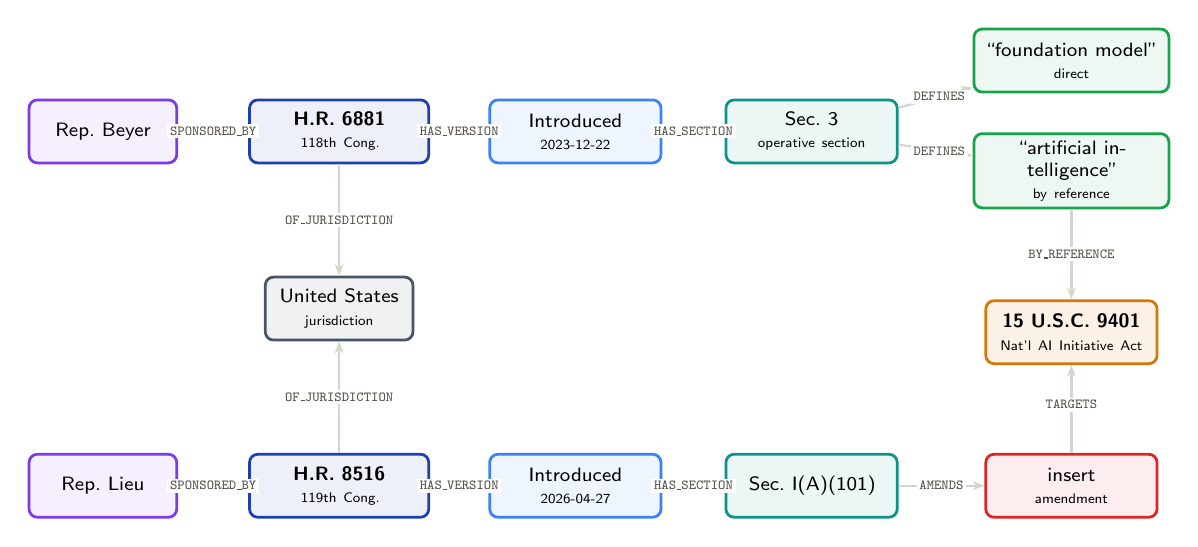
\begin{tikzpicture}[
  font=\sffamily\scriptsize,
  every node/.style={align=center},
  N/.style={draw,rounded corners=3pt,minimum height=0.8cm,text width=2.0cm,
    inner sep=2.5pt,line width=1pt},
  bill/.style={N,draw=cBill,fill=cBill!8,text width=2.1cm},
  ver/.style={N,draw=cVer,fill=cVer!8},
  sec/.style={N,draw=cSec,fill=cSec!8},
  term/.style={N,draw=cTerm,fill=cTerm!8,text width=2.3cm},
  stat/.style={N,draw=cStat,fill=cStat!10},
  amend/.style={N,draw=cAmend,fill=cAmend!8},
  spon/.style={N,draw=cSpon,fill=cSpon!8,text width=1.7cm},
  jur/.style={N,draw=cJur,fill=cJur!8,text width=1.7cm},
  e/.style={-{Stealth[length=1.5mm]},rule,line width=0.8pt},
  el/.style={font=\ttfamily\tiny,text=ink2,fill=white,inner sep=1pt}]

% --- H.R. 6881 cluster (top) ---
\node[spon] (s1) at (0,3.1) {Rep.\ Beyer};
\node[bill] (b1) at (3,3.1) {\textbf{H.R.\ 6881}\\\tiny 118th Cong.};
\node[ver]  (v1) at (6,3.1) {Introduced\\\tiny 2023-12-22};
\node[sec]  (c1) at (9,3.1) {Sec.\ 3\\\tiny operative section};
\node[term] (t1) at (12.3,4.0) {``foundation model''\\\tiny direct};
\node[term] (t2) at (12.3,2.6) {``artificial intelligence''\\\tiny by reference};

% --- shared statute (middle right) ---
\node[stat] (ss) at (12.3,0.55) {\textbf{15 U.S.C.\ 9401}\\\tiny Nat'l AI Initiative Act};

% --- H.R. 8516 cluster (bottom) ---
\node[spon] (s2) at (0,-1.4) {Rep.\ Lieu};
\node[bill] (b2) at (3,-1.4) {\textbf{H.R.\ 8516}\\\tiny 119th Cong.};
\node[ver]  (v2) at (6,-1.4) {Introduced\\\tiny 2026-04-27};
\node[sec]  (c2) at (9,-1.4) {Sec.\ I(A)(101)};
\node[amend](am) at (12.3,-1.4) {insert\\\tiny amendment};

% --- jurisdiction ---
\node[jur] (j) at (3,0.85) {United States\\\tiny jurisdiction};

% edges, H.R. 6881
\draw[e] (s1) -- (b1) node[el,midway]{SPONSORED\_BY};
\draw[e] (b1) -- (v1) node[el,midway]{HAS\_VERSION};
\draw[e] (v1) -- (c1) node[el,midway]{HAS\_SECTION};
\draw[e] (c1) -- (t1) node[el,pos=0.55]{DEFINES};
\draw[e] (c1) -- (t2) node[el,pos=0.55]{DEFINES};
\draw[e] (t2) -- (ss) node[el,pos=0.5]{BY\_REFERENCE};
\draw[e] (b1) -- (j)  node[el,pos=0.5]{OF\_JURISDICTION};
% edges, H.R. 8516
\draw[e] (s2) -- (b2) node[el,midway]{SPONSORED\_BY};
\draw[e] (b2) -- (v2) node[el,midway]{HAS\_VERSION};
\draw[e] (v2) -- (c2) node[el,midway]{HAS\_SECTION};
\draw[e] (c2) -- (am) node[el,midway]{AMENDS};
\draw[e] (am) -- (ss) node[el,pos=0.55]{TARGETS};
\draw[e] (b2) -- (j)  node[el,pos=0.5]{OF\_JURISDICTION};
\end{tikzpicture}
\caption{Two real bills, one shared statute. \textbf{H.R.~6881} borrows its
definition of ``artificial intelligence'' from \textbf{15~U.S.C.~9401}
(\code{BY\_REFERENCE}); \textbf{H.R.~8516} rewrites that same section
(\code{AMENDS} $\rightarrow$ \code{TARGETS}). Two bills that share no sponsor,
no Congress and no keyword are bound together through one statute node --- and
the graph finds that link in a single hop. The companion file
\code{polilabs-graph.html} is this figure, live and clickable.}
\label{fig:graph}
\end{figure}

This is the payoff of the whole architecture. ``Which bills touch the
definition of AI that Congress enacted in 2020?'' is, against a pile of XML, a
research project. Against the graph it is one query: find
\code{15 U.S.C. 9401}, follow every \code{BY\_REFERENCE} and \code{TARGETS}
edge backwards.

% =================================================================
\section{The MCP and the agent tools}

\subsection{What ``MCP'' means here}

MCP --- the Model Context Protocol --- is a standard way to expose a set of
\emph{tools} to an LLM. A tool is a named function with a typed schema: the
model sees ``here is a function \code{search\_corpus(query, tier, limit)}'',
decides to call it, and gets a structured result back.

polilabs ships an MCP server (\code{mcp\_server.py}). Point Claude Desktop,
Cursor, or any MCP client at it and that client's model gains 12 new tools for
querying federal AI legislation. The MCP server needs no API key of its own ---
it only reads the two local stores; the LLM is supplied by the client.

Critically, \textbf{the same 12 tools back four different front doors}: the MCP
server, an HTTP/SSE web API, a terminal REPL, and the evaluation harness. They
all import one tool catalogue and one system prompt from \code{agent/tools.py}.
Write a tool once, get it everywhere.

\subsection{The twelve tools}

\begin{table}[ht]
\centering\footnotesize
\begin{tabular}{@{}lp{8.0cm}l@{}}
\toprule
\textbf{Tool} & \textbf{What it does} & \textbf{Store}\\
\midrule
\multicolumn{3}{@{}l}{\itshape\color{ink2} Discovery \& scope}\\
\code{search\_corpus}      & Free-text search; ranked bill hits + a hint that routes to aggregate tools & SQLite\\
\code{corpus\_coverage}    & What is in and out of scope --- the ``say I don't know'' tool & SQLite\\
\midrule
\multicolumn{3}{@{}l}{\itshape\color{ink2} Single-bill drill-in}\\
\code{get\_bill}           & Metadata + a table of contents (no body text) & SQLite\\
\code{get\_section}        & Verbatim section text + its canonical citation & SQLite + graph\\
\code{get\_defined\_terms} & Every term one bill formally defines & graph\\
\code{get\_amendments}     & Every amendment one bill makes to existing law & graph\\
\midrule
\multicolumn{3}{@{}l}{\itshape\color{ink2} Cross-reference \& targeting}\\
\code{get\_citation\_graph}     & The typed citation graph around a section & graph\\
\code{get\_amendments\_targeting} & Every amendment in the corpus hitting one US Code section & graph\\
\code{resolve\_citation}        & ``Sec.\ 3(a) of H.R.\ 1736'' $\rightarrow$ a canonical section id & SQLite\\
\midrule
\multicolumn{3}{@{}l}{\itshape\color{ink2} Aggregate --- ``list every bill that\ldots'' (one call, not fifty)}\\
\code{find\_bills\_defining}  & Every bill defining a given term & graph\\
\code{find\_bills\_amending}  & Per-bill rollup of bills amending a US Code section & graph\\
\code{find\_definitions\_of}  & Every bill's verbatim definition of a term, side by side & graph\\
\bottomrule
\end{tabular}
\caption{The agent tool surface. The four \emph{aggregate} tools were added
after evaluation revealed that agents systematically truncate
``search-then-loop'' patterns at roughly 20 sequential calls --- so the
expensive multi-step pattern was collapsed into a single primitive.}
\end{table}

\subsection{How a tool call is implemented}

Every tool is the thin top of a three-layer stack:

\begin{enumerate}[leftmargin=1.5em,itemsep=2pt]
\item \textbf{Tool wrapper} (\code{agent/tools.py}) --- accepts plain JSON
  arguments, validates and clamps them, calls the primitive below, and
  serializes the result to a JSON string. Errors become structured
  \code{\{"error": \ldots\}} objects; the agent never sees a stack trace.
\item \textbf{Typed primitive} (\code{api/\_impl.py}) --- the real query logic.
  It runs SQL against SQLite, or Cypher against the K\`uzu graph, or both, and
  returns a typed Python object.
\item \textbf{Storage} --- the SQLite FTS index and the K\`uzu graph.
\end{enumerate}

The contract for that middle layer is written down in \code{api/SPEC.md}, and
its invariants are themselves anti-hallucination rules. Three of the nine: every
chunk of verbatim text is returned \emph{with} its canonical citation, so the
agent never reconstructs a citation; an empty result is always distinguishable
from an out-of-scope result; and a primitive \emph{never} raises on ``not found''
--- it returns a typed answer that says so.

% =================================================================
\section{End to end: a question becomes an answer}

Putting it together --- here is what happens when a researcher asks, through the
web front end, \emph{``How does each bill define `foundation model'?''}

\begin{figure}[ht]
\centering
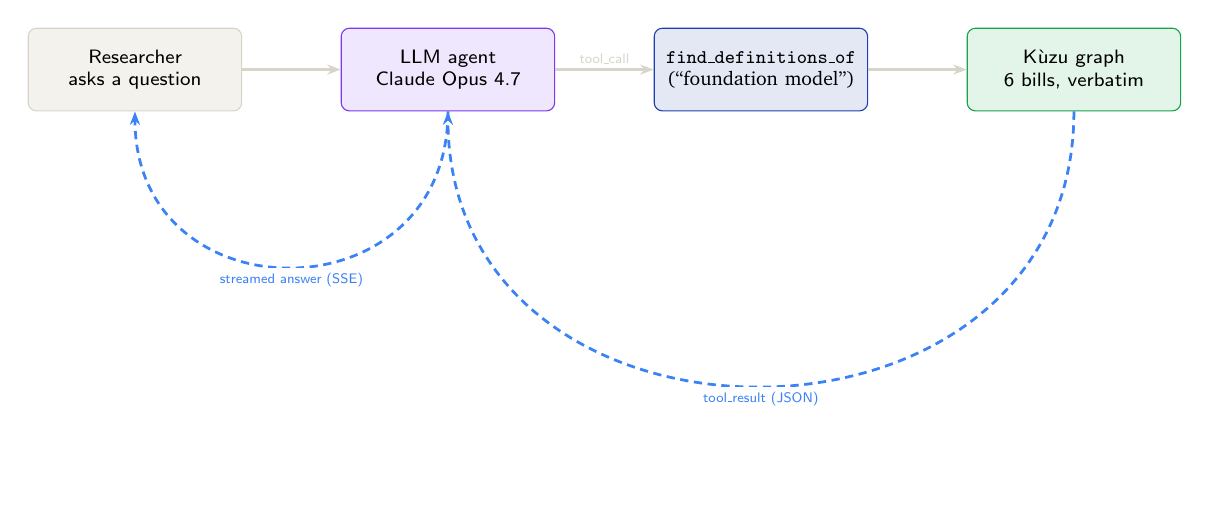
\begin{tikzpicture}[
  font=\sffamily\scriptsize,
  box/.style={draw=rule,fill=panel,rounded corners=3pt,minimum height=1.05cm,
    text width=2.5cm,align=center,inner sep=3pt},
  agentb/.style={box,fill=cSpon!12,draw=cSpon},
  toolb/.style={box,fill=cBill!12,draw=cBill,text width=2.5cm},
  graphb/.style={box,fill=cTerm!12,draw=cTerm},
  fwd/.style={-{Stealth[length=1.7mm]},rule,line width=1pt},
  ret/.style={-{Stealth[length=1.7mm]},cVer,line width=1pt,densely dashed},
  lab/.style={font=\sffamily\tiny,fill=white,inner sep=1.6pt},
  node distance=1.25cm]
\node[box] (user) {Researcher\\asks a question};
\node[agentb,right=of user] (agent) {LLM agent\\Claude Opus 4.7};
\node[toolb,right=of agent] (tool) {\ttfamily\scriptsize find\_definitions\_of\\\normalfont(``foundation model'')};
\node[graphb,right=of tool] (graph) {K\`uzu graph\\6 bills, verbatim};
\draw[fwd] (user) -- (agent);
\draw[fwd] (agent) -- (tool) node[lab,midway,above]{tool\_call};
\draw[fwd] (tool) -- (graph);
\draw[ret] (graph) to[out=-90,in=-90,looseness=1.5]
  node[lab,midway,below]{tool\_result (JSON)} (agent);
\draw[ret] (agent) to[out=-90,in=-90,looseness=1.7]
  node[lab,midway,below]{streamed answer (SSE)} (user);
\end{tikzpicture}
\caption{The chat path. The agent loop runs until the model stops calling
tools; the server streams every step.}
\label{fig:flow}
\end{figure}

\begin{enumerate}[leftmargin=1.5em,itemsep=3pt]
\item The question hits the \code{POST /chat} endpoint. The server starts an
  agent loop with \textbf{Claude Opus 4.7} and the 12 tools.
\item The system prompt tells the agent: for any ``which bills do X'' question,
  do \emph{not} search then loop --- go straight to an aggregate tool. So the
  agent calls \code{find\_definitions\_of("foundation model")}.
\item That one call runs a single graph query and returns every bill's
  \emph{verbatim} definition of the term --- six of them --- side by side.
\item The agent writes the answer, quoting the definitions and their canonical
  citations exactly as the tool returned them. It cannot drift, because it never
  had the raw text in any other form.
\item The whole run streams to the browser as Server-Sent Events:
  \code{text} (answer prose), \code{tool\_call} (a tool was invoked),
  \code{tool\_result} (structured data, so the UI can render panels),
  \code{done}, \code{error}. The front end renders the answer and the sources
  as they arrive.
\end{enumerate}

The web front end also has a second, cheaper path: a set of read-only
\code{GET /api/*} REST endpoints that wrap nine of the tools directly. Clicking
between bills in the UI uses those --- no LLM, no token cost, instant.

% =================================================================
\section{Who uses this, and how}

The machine above only matters if it shortens real work. This section is for
the reader with no policy background.

\subsection{A sixty-second primer on bills}

A \textbf{bill} is a proposed law. A member of the House introduces an ``H.R.''
bill; a Senator introduces an ``S.'' bill; each gets a number (H.R.~6881). It
is referred to a committee. \emph{Most bills die there} --- they are never voted
on. A few are amended (``marked up''), voted out of committee, passed by the
full chamber, sent to the other chamber, and --- rarely --- signed into law.

Two facts shape the research problem:

\begin{itemize}[leftmargin=1.4em,itemsep=2pt]
\item \textbf{Congresses are two years long and bills do not survive them.} The
  118th Congress was 2023--24; the 119th is 2025--26. A bill not passed by the
  end of its Congress is dead and must be reintroduced from scratch --- often
  with a new number and slightly changed text. So the ``landscape'' on any
  topic is dozens of overlapping, competing, reintroduced drafts.
\item \textbf{Bills mostly edit existing law.} A bill rarely writes a statute
  from a blank page. It \emph{amends} the US Code --- ``strike subsection (b)
  and insert the following''. To understand a bill you must understand what it
  changes. And bills \textbf{define their own terms}: ``artificial
  intelligence'' means whatever \emph{this} bill's definitions section says, and
  the next bill may say something different.
\end{itemize}

That last point is why polilabs scopes definitions to bills and never builds a
global ``AI'' node. The disagreement between definitions \emph{is} the research
finding.

\subsection{Who does this work}

\begin{table}[ht]
\centering\small
\begin{tabular}{@{}lp{9.0cm}@{}}
\toprule
\textbf{User} & \textbf{What they need from legislative research}\\
\midrule
Congressional staff & Legislative assistants and committee staff drafting a
  bill: what else has been introduced on this topic, who sponsored it, what it
  does, what it would amend --- so they do not duplicate or contradict.\\
CRS analysts & The Congressional Research Service is Congress's in-house,
  nonpartisan research arm. It writes side-by-side comparisons of legislative
  approaches for members of both parties.\\
Government affairs / lobbyists & Track every bill that could affect a client or
  industry; need early warning and precise, defensible analysis.\\
Think tanks \& academics & Groups like CSET, Brookings, or Stanford HAI publish
  ``the state of federal AI legislation'' reports --- exactly a literature
  review over bills.\\
Corporate policy \& compliance & AI companies especially: what regulation is
  coming, how would each bill's definitions catch (or exempt) our products.\\
Journalists \& advocacy orgs & Cover or campaign on specific bills; need to get
  the facts and citations exactly right.\\
\bottomrule
\end{tabular}
\caption{The audience. All of them do some version of the same task below.}
\end{table}

\subsection{How a policy researcher does a bill literature review}

Suppose a researcher is asked: \emph{``Give us the landscape of how federal AI
bills define and regulate `foundation models'.''} Today, without polilabs, the
work runs roughly like this:

\begin{enumerate}[leftmargin=1.6em,itemsep=3pt]
\item \textbf{Scope.} Pin down the question --- which Congresses, which sense of
  the term, what counts as ``in''.
\item \textbf{Discover.} Search Congress.gov (free, official) or a paid
  platform --- Bloomberg Government, POLITICO Pro, Quorum, FiscalNote --- by
  keyword, policy area, and subject. This returns a long, noisy list.
\item \textbf{Triage.} Read each title and its official summary; skim; cull the
  list to what is genuinely relevant. Slow, and judgment-heavy.
\item \textbf{Deep read.} Pull the full text of each surviving bill. Find the
  definitions section. Find the operative sections. Work out what existing law
  it amends.
\item \textbf{Compare.} Build a comparison --- almost always a spreadsheet:
  one row per bill, columns for the definition, the threshold, the scope, the
  enforcing agency, the penalties. This matrix \emph{is} the deliverable, and
  building it is entirely manual.
\item \textbf{Write up.} Turn the matrix into a memo, with every bill and
  section cited exactly --- because a wrong citation discredits the whole
  document.
\end{enumerate}

The pain is concentrated in steps 3--6. Keyword search (step~2) silently misses
bills that use a different phrase. Because every bill defines terms locally
(step~4), the comparison in step~5 is apples-to-oranges by construction --- you
cannot compare ``foundation model'' across bills until you have read each bill's
own definition. And step~6 is where general-purpose AI tools fail worst: asked
to summarize, they hallucinate citations.

\subsection{Where polilabs fits}

polilabs is not a chat-with-a-PDF wrapper bolted onto this workflow. It replaces
the \emph{substrate} the workflow runs on, so that steps 2--5 become tool calls
an agent makes in seconds:

\begin{itemize}[leftmargin=1.4em,itemsep=2pt]
\item Discovery and triage (steps 2--3) $\rightarrow$ \code{search\_corpus},
  with a curated corpus that already applied the inclusion test.
\item The comparison matrix (step~5) $\rightarrow$
  \code{find\_definitions\_of("foundation model")} returns every bill's
  verbatim definition side by side --- the spreadsheet, in one call.
\item ``What does each bill change about existing law'' $\rightarrow$
  \code{get\_amendments} and \code{find\_bills\_amending}.
\item The write-up (step~6) is safe \emph{by construction}: every definition,
  every citation the agent reports came verbatim from a tool result, carrying
  its own provenance. The agent can also say, honestly, ``executive orders are
  outside this corpus'' instead of guessing.
\end{itemize}

The researcher still does the thinking --- scoping the question, judging
significance, writing the argument. polilabs removes the mechanical
substrate-fighting in the middle, and removes the hallucination risk at the end.

% =================================================================
\section{Honest status --- what is built, what is not}

This document describes a v1 that genuinely works, but it would be misleading
to imply it is finished.

\textbf{What works.} All 191 bills are ingested, parsed, and indexed into both
stores with zero parse errors. All 12 tools are implemented and live across all
four transports. The evaluation harness --- 13 hand-curated queries scored for
both under-coverage and over-confidence --- passes \textbf{12 of 13}, with zero
hallucinated citations; the one failure is model variance on a stylistic check,
not a code bug.

\textbf{What is stubbed.} The schema design document (\code{schema\_design.md})
specifies a far larger ontology --- 23 node types, interpretive-reasoning nodes,
bitemporal versioning, soft ``conflicts-with'' edges, an enactment-version
synthesizer. The \emph{implemented} graph is the mechanical subset: ten
populated node types, twelve populated edge types. Three declared node types
(\code{Committee}, \code{Statute}, \code{UnresolvedTermUse}) and four edge types
are not yet populated. Treat \code{schema\_design.md} as the roadmap and this
document as the territory.

\textbf{Known limits.} v1 stores one canonical version per bill --- the schema
supports a full version history, but it is not wired. Amendment ``before''
text is marked unverified, because the US Code itself is not yet ingested for
comparison. The two USLM-format bills produce no citation edges (a parser gap).
And the corpus is, deliberately, only AI-governance legislation --- not all of
federal law.

None of this undercuts the v1 thesis. It bounds it: polilabs v1 is a working,
honest, anti-hallucination research substrate for one well-defined corpus, with
a clear path to more.

\vspace{0.6cm}
\sectionrule
\begin{center}\small\color{ink2}
Companion: open \code{polilabs-graph.html} for the interactive graph.\\
Source of every number here: the v1 corpus and the indexes built from it.
\end{center}

\end{document}
